\documentclass[aspectratio=169,professionalfonts,12pt]{beamer}
\usepackage[T1]{fontenc}
\usepackage{lmodern,microtype}
\usepackage{amsmath,amssymb,booktabs,tabularx,array,colortbl,makecell}
\usepackage{tikz}
\usetikzlibrary{arrows.meta,positioning,calc,backgrounds,fit}
\usepackage{hyperref}
\usepackage{verbatim}
\usepackage{transparent}

\definecolor{navy}{HTML}{16324F}
\definecolor{copper}{HTML}{B35C1E}
\definecolor{teal}{HTML}{277C78}
\definecolor{blue}{HTML}{0072B2}
\definecolor{ice}{HTML}{EDF4F7}
\definecolor{warm}{HTML}{F7F0E9}
\definecolor{ink}{HTML}{20262E}
\definecolor{muted}{HTML}{5C6773}
\definecolor{pale}{HTML}{F7F9FA}
\definecolor{good}{HTML}{168C55}
\definecolor{maybe}{HTML}{C99100}
\definecolor{bad}{HTML}{C7352C}
\definecolor{TitleBlue}{HTML}{123A63}
\definecolor{CircuitBlue}{HTML}{A9D5E8}

\let\olditemize\itemize
\let\endolditemize\enditemize

\usepackage{etoolbox}
\usepackage{xcolor}

\BeforeBeginEnvironment{itemize}{\vspace{0.3em}}
\AtBeginEnvironment{itemize}{%
  \setlength{\itemsep}{0.3em}%
}
\AfterEndEnvironment{itemize}{\vspace{0.3em}}

\usetikzlibrary{circuits.ee.IEC}
\usetikzlibrary{overlay-beamer-styles}
\usetikzlibrary{positioning}
\usetikzlibrary{calc,patterns}
\usepackage{circuitikz}

\usetikzlibrary{patterns}
\setcounter{MaxMatrixCols}{12}

% One dot per 0.8 mm square.
\pgfdeclarepatternformonly{weightdots}
{\pgfpoint{0pt}{0pt}}
{\pgfpoint{0.8mm}{0.8mm}}
{\pgfpoint{0.8mm}{0.8mm}}
{%
  \pgfpathcircle
  {\pgfpoint{0.4mm}{0.4mm}}
  {0.1mm}
  \pgfusepath{fill}
}

% Fixed-size equals sign and labels, independent of surrounding math size.
\newcommand{\slideequals}{%
  \mathrel{\text{\normalsize$=$}}%
}
\newcommand{\slidelabel}[1]{%
  \text{\small #1}%
}

% From the TeX.SE answer:
% https://tex.stackexchange.com/questions/6135/how-to-make-beamer-overlays-with-tikz-node
\tikzset{
  onslide/.code args={<#1>#2}{%
    \only<#1>{\pgfkeysalso{#2}}%
  }
}

\usetheme{default}
\usefonttheme{professionalfonts}
\setbeamercolor{normal text}{fg=ink,bg=white}
\setbeamercolor{structure}{fg=navy}
\setbeamercolor{frametitle}{fg=navy,bg=white}
\setbeamercolor{title}{fg=navy}
\setbeamercolor{subtitle}{fg=teal}
\setbeamercolor{alerted text}{fg=copper}
\setbeamercolor{block title}{fg=white,bg=navy}
\setbeamercolor{block body}{fg=ink,bg=ice}
\setbeamerfont{title}{size=\fontsize{24}{28},series=\bfseries}
\setbeamerfont{frametitle}{size=\fontsize{22}{26},series=\bfseries}
\setbeamerfont{subtitle}{size=\large}
\setbeamertemplate{navigation symbols}{}
\setbeamertemplate{itemize item}{\color{copper}$\blacktriangleright$}
\setbeamertemplate{itemize subitem}{\color{teal}$\bullet$}
\setbeamersize{text margin left=1cm,text margin right=1cm}
\setbeamertemplate{frametitle}{\vspace{2.5mm}\hspace{-2.5mm}\insertframetitle\par\vspace{-2mm}{\hspace{-2.5mm}\color{copper}\rule{\dimexpr \textwidth + 2.5mm \relax}{0.8pt}}}
\setbeamertemplate{footline}{\leavevmode\hbox{%
    \begin{beamercolorbox}[wd=.95\paperwidth,ht=2.5ex,dp=1.0ex]{normal text}\end{beamercolorbox}%
    \begin{beamercolorbox}[wd=.05\paperwidth,ht=2.5ex,dp=1.0ex,rightskip=5mm plus1fil]{normal text}\color{muted}\scriptsize \insertframenumber/\inserttotalframenumber\end{beamercolorbox}}
  \vspace{2mm}}

\begin{document}

\newcommand{\yes}{\textcolor{good}{\bfseries\checkmark}}
\newcommand{\partly}{\textcolor{maybe}{\bfseries---}}
\newcommand{\no}{\textcolor{bad}{\bfseries$\times$}}
\newcommand{\source}[1]{\par\vfill\nointerlineskip{\color{muted}\tiny #1\par}}
\newcolumntype{C}{>{\centering\arraybackslash}X}

\title{\textbf{Ohm Improvement:}\\Programming for Drift Tolerance in\\Computational Phase-Change Memory}
\author{Peter Coffman}
\date{17 August 2026}

\begin{frame}[plain]
  \begin{tikzpicture}[remember picture,overlay]
    % Decorative PCM crossbar array. The scope is intentionally rotated
    % 12.5 degrees from vertical and clipped by the slide edge.
    \begin{scope}[
      shift={([xshift=5.85cm,yshift=-0.10cm]current page.center)},
      rotate=12.5,
      draw=CircuitBlue,
      line width=0.22pt,
      opacity=0.62,
      line cap=round,
      line join=round
      ]
      % Word lines and their faint driver stubs.
      \foreach \r in {-4.2,-3.35,...,4.3} {
        \draw (-4.4,\r) -- (4.25,\r);
        \draw (-4.75,\r-0.17) -- (-4.4,\r) -- (-4.75,\r+0.17) -- cycle;
      }

      % Bit lines and terminal pads.
      \foreach \c in {-3.5,-2.65,...,3.3} {
        \draw (\c,-4.75) -- (\c,4.75);
        \draw (\c-0.11,4.75) rectangle (\c+0.11,5.02);
      }

      % Stylized 1T1R / PCM cells at the intersections.
      \foreach \c in {-3.5,-2.65,...,3.3} {
        \foreach \r in {-4.2,-3.35,...,4.3} {
          \draw (\c-0.20,\r) -- (\c-0.12,\r);
          \draw (\c-0.12,\r-0.12) rectangle (\c+0.12,\r+0.12);
          \draw (\c+0.12,\r) -- (\c+0.20,\r);
          \fill[CircuitBlue] (\c,\r) circle (0.024);
        }
      }

      % Sparse peripheral traces suggest row/column addressing without
      % competing with the title.
      \draw (-4.95,-4.55) -- (-4.95,4.55);
      \draw (-5.12,-3.95) -- (-4.95,-3.95);
      \draw (-5.12,-1.40) -- (-4.95,-1.40);
      \draw (-5.12, 1.15) -- (-4.95, 1.15);
      \draw (-5.12, 3.70) -- (-4.95, 3.70);
      \draw (-3.90, 5.22) -- (3.70, 5.22);
    \end{scope}

    \node[
    anchor=west,
    text=TitleBlue,
    text width=11.4cm,
    align=left
    ] at ([xshift=1.18cm,yshift=0.55cm]current page.west) {%
      {\fontsize{29}{34}\selectfont\bfseries
        Ohm Improvement\par}
      \vspace{0.42cm}
      {\fontsize{12.8}{16.2}\selectfont
        Programming for Drift Tolerance in\\Computational Phase-Change Memory\par}
    };

    \node[
    anchor=west,
    text=TitleBlue
    ] at ([xshift=1.18cm,yshift=-3.00cm]current page.west) {%
      {\fontsize{9.5}{12}\selectfont Peter Coffman\enspace|\enspace \today}%
    };
  \end{tikzpicture}
\end{frame}

\begin{frame}{AI is expensive}
  \begin{columns}[T,onlytextwidth]
    \begin{column}{0.3\textwidth}
      \uncover<2->{
        \centering
        \textbf{Power}\par
        \begin{minipage}[c][5cm][c]{\linewidth}
          \centering
          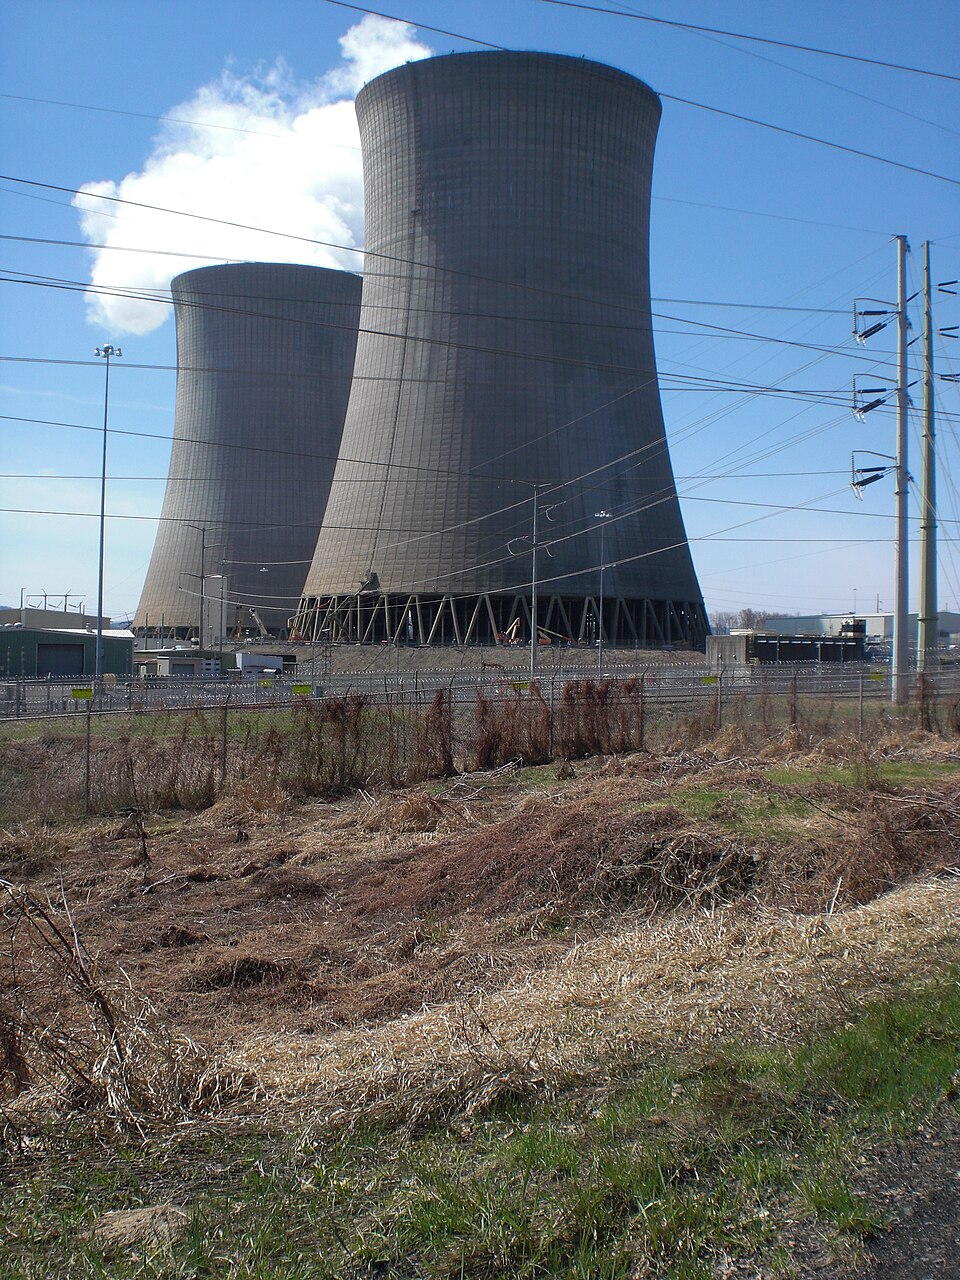
\includegraphics[
          width=\linewidth,height=4cm,keepaspectratio
          ]{figures/Susquehanna.JPG}
        \end{minipage}\par
        {\fontsize{6}{8}\selectfont
          Photo: Jakec; edit: Crisco 1492 /
          Wikimedia Commons / CC BY-SA 4.0.\par}
      }
    \end{column}

    \begin{column}{0.3\textwidth}
      \uncover<3->{
        \centering
        \textbf{Hardware}\par
        \begin{minipage}[c][5cm][c]{\linewidth}
          \centering
          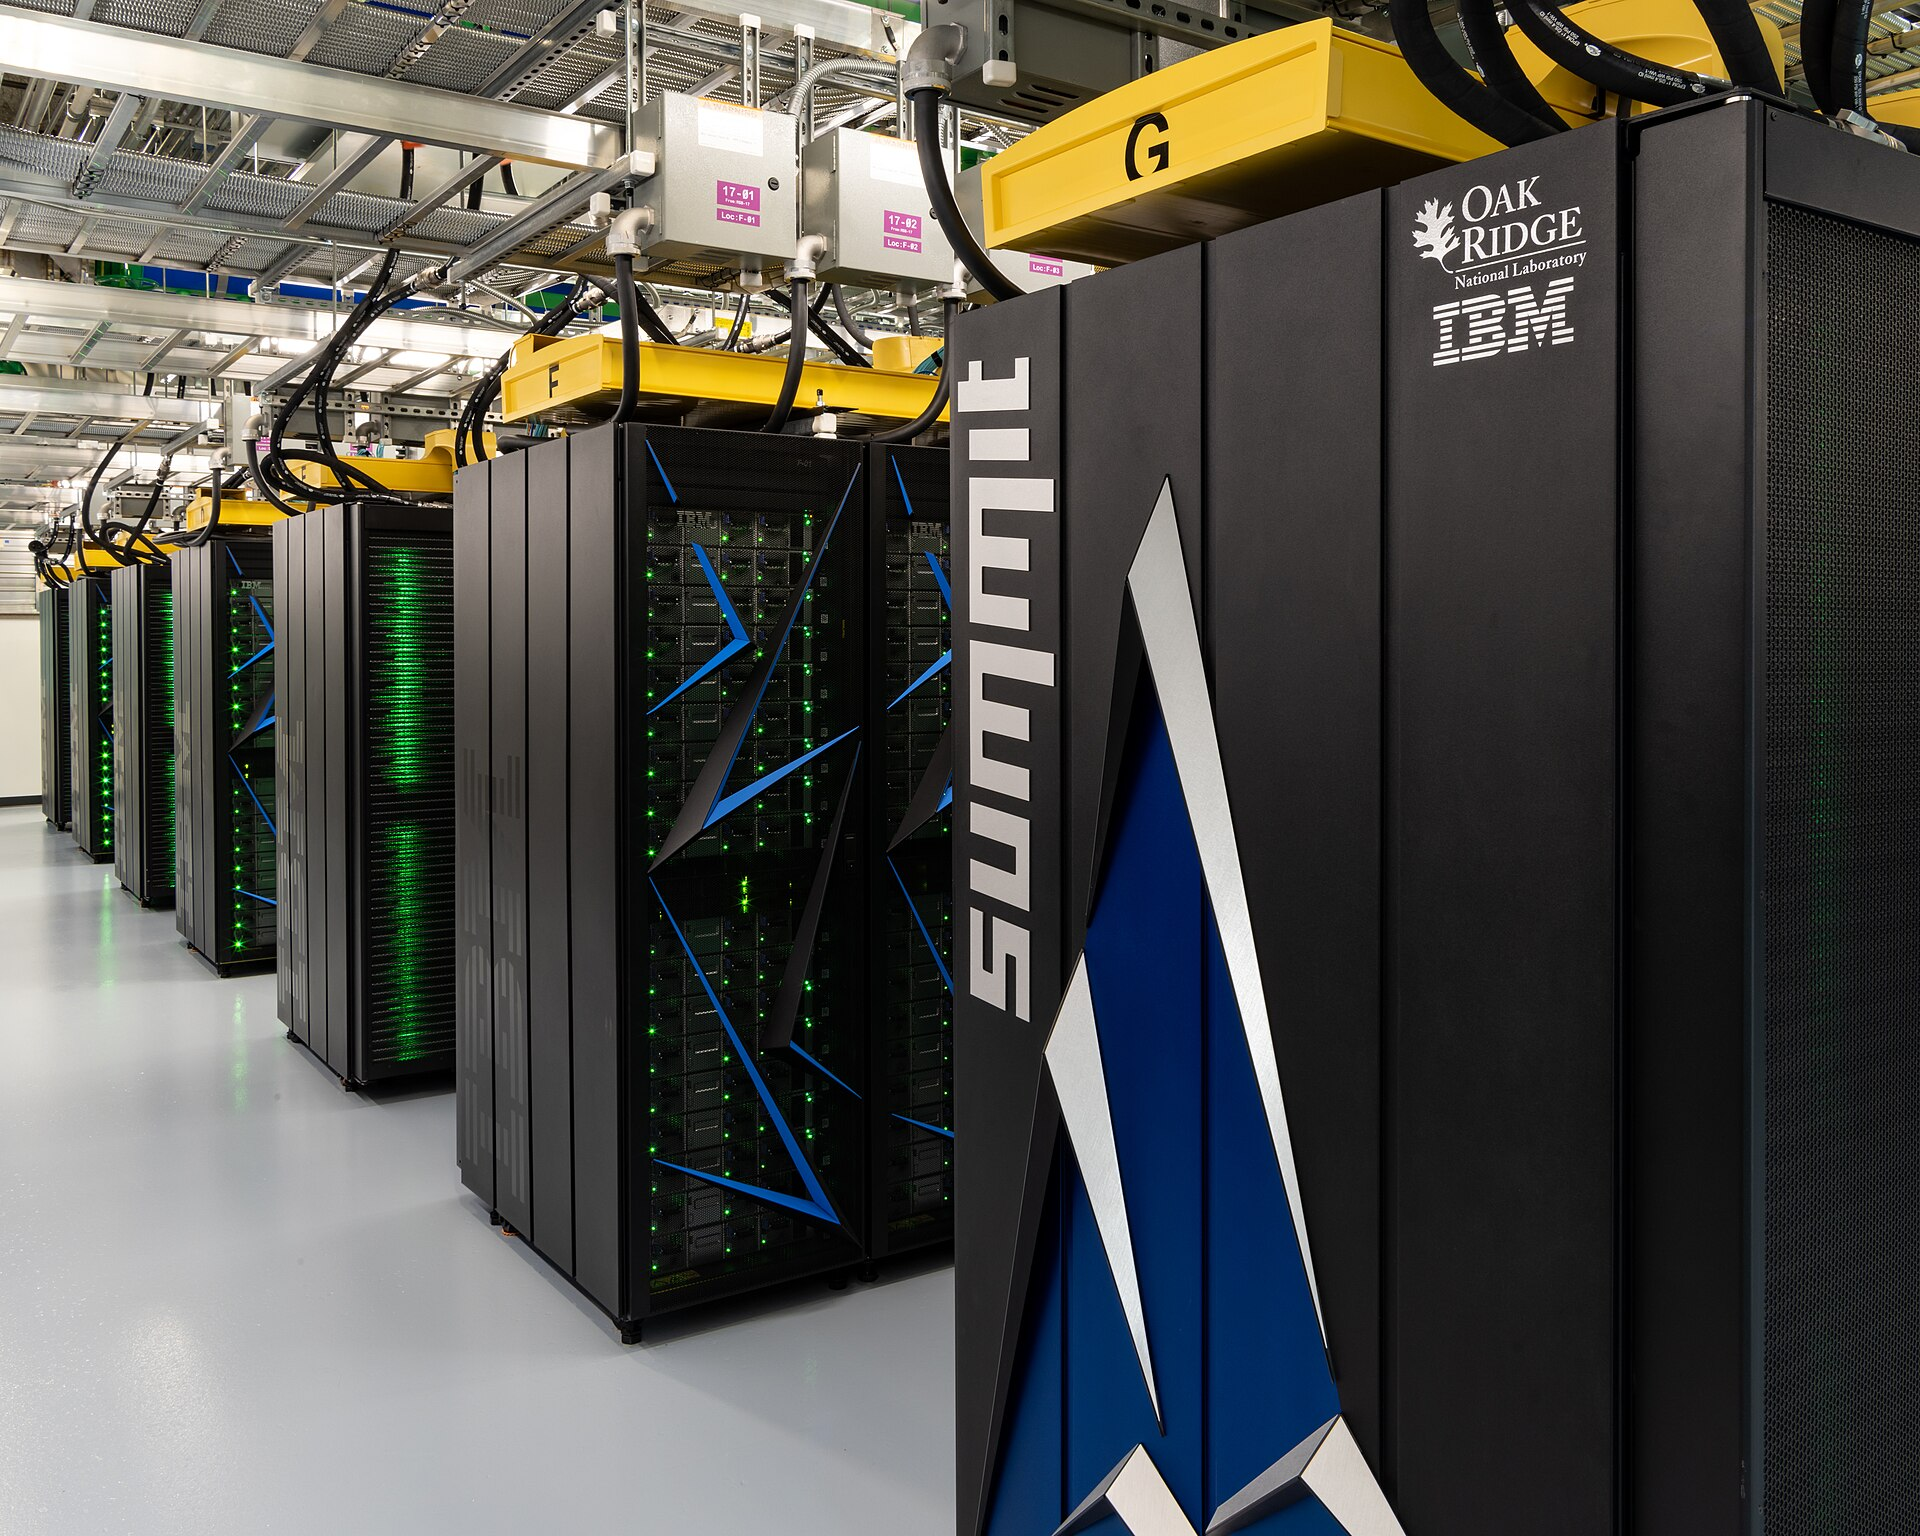
\includegraphics[
          width=\linewidth,height=4cm,keepaspectratio
          ]{figures/Summit_(supercomputer).jpg}
        \end{minipage}\par
        {\fontsize{6}{8}\selectfont
          Photo: Carlos Jones/ORNL / CC BY 2.0.\par}
      }
    \end{column}

    \begin{column}{0.3\textwidth}
      \uncover<4->{
        \centering
        \textbf{Time}\par
        \begin{minipage}[c][5cm][c]{\linewidth}
          \centering
          
\includegraphics[
          width=\linewidth,height=4cm,keepaspectratio
          ]{figures/working.png}
        \end{minipage}\par
        {\fontsize{6}{8}\selectfont
          Screenshot: OpenAI ChatGPT,
          captured by the author.\par}
      }
    \end{column}
  \end{columns}
\end{frame}

\begin{frame}{Why is AI expensive?}
  \begin{overlayarea}{\textwidth}{6.2cm}
    \centering

    \only<2-4>{%
      \vspace*{2.5mm}
      Mostly one operation: \textit{Matrix-Vector Multiplication (MVM)}
    }

    % ----------------------------------------------------------
    % Overlay 2: 2 rows, 2 columns.
    % ----------------------------------------------------------
    \only<3-4>{%
      \normalsize
      \begin{align*}
        (\textcolor{copper}{2}\times\textcolor{blue}{3})
        +(\textcolor{copper}{4}\times\textcolor{blue}{1})
        &\slideequals 10\\
        (\textcolor{copper}{1}\times\textcolor{blue}{3})
        +(\textcolor{copper}{3}\times\textcolor{blue}{1})
        &\slideequals 6\\
        \\
        \only<4>{\underset{\slidelabel{stored weights}}{
        \textcolor{copper}{
        \begin{bmatrix}
          2 & 4\\
          1 & 3
        \end{bmatrix}
        }
        }
        \quad
        \underset{\slidelabel{inputs}}{
        \textcolor{blue}{
        \begin{bmatrix}3\\1\end{bmatrix}
        }
        }
        &\slideequals
          \underset{\slidelabel{outputs}}{
          \begin{bmatrix}10\\6\end{bmatrix}
          }
          }
      \end{align*}

      \vspace{-2mm}
      \only<4>{\small 4 stored weights\par}
    }

    % ----------------------------------------------------------
    % Overlay 5: 12 rows, 12 columns.
    % ----------------------------------------------------------
    \only<5>{%
      \begingroup
      \scriptsize
      \setlength{\arraycolsep}{3pt}
      \renewcommand{\arraystretch}{0.90}
      \setlength{\abovedisplayskip}{3pt}
      \setlength{\belowdisplayskip}{3pt}

      % Arithmetic for the first output.
      \[
        \begin{aligned}
          &(\textcolor{copper}{1}\times\textcolor{blue}{3})
            +(\textcolor{copper}{0}\times\textcolor{blue}{5})
            +(\textcolor{copper}{4}\times\textcolor{blue}{5})
            +(\textcolor{copper}{3}\times\textcolor{blue}{2})
            +(\textcolor{copper}{3}\times\textcolor{blue}{2})
            +(\textcolor{copper}{2}\times\textcolor{blue}{3})
          \\
          &\quad
            +(\textcolor{copper}{1}\times\textcolor{blue}{2})
            +(\textcolor{copper}{8}\times\textcolor{blue}{5})
            +(\textcolor{copper}{1}\times\textcolor{blue}{5})
            +(\textcolor{copper}{9}\times\textcolor{blue}{1})
            +(\textcolor{copper}{6}\times\textcolor{blue}{5})
            +(\textcolor{copper}{0}\times\textcolor{blue}{3})
            \slideequals 127
        \end{aligned}
      \]

      \[
        \underset{\slidelabel{stored weights}}{
          \textcolor{copper}{
            \begin{bmatrix}
              1&0&4&3&3&2&1&8&1&9&6&0\\
              0&1&3&3&8&9&0&8&3&8&6&3\\
              7&9&4&0&2&6&5&4&2&3&5&1\\
              1&6&1&5&5&9&4&0&7&8&1&6\\
              1&8&4&9&5&9&3&1&0&3&4&1\\
              3&1&6&4&7&5&2&5&5&3&4&1\\
              9&2&8&3&2&7&6&4&8&3&5&0\\
              3&0&5&6&4&1&3&9&5&3&7&6\\
              7&2&4&2&3&8&8&4&9&6&9&6\\
              5&3&2&8&7&1&0&1&2&2&6&9\\
              1&6&6&9&7&8&4&8&0&1&8&4\\
              5&1&4&6&2&7&0&4&8&2&8&1
            \end{bmatrix}
          }
        }
        \quad
        \underset{\slidelabel{inputs}}{
          \textcolor{blue}{
            \begin{bmatrix}
              3\\5\\5\\2\\2\\3\\2\\5\\5\\1\\5\\3
            \end{bmatrix}
          }
        }
        \slideequals
        \underset{\slidelabel{outputs}}{
          \begin{bmatrix}
            127\\171\\179\\159\\155\\161\\
            208\\189\\235\\147\\220\\182
          \end{bmatrix}
        }
      \]
      \endgroup

      \smallskip
      {\small 144 stored weights\par}
    }

    % ----------------------------------------------------------
    % Overlay 6: 64 rows, 64 columns.
    % ----------------------------------------------------------
    \only<6>{%
      \vspace*{-2mm}
      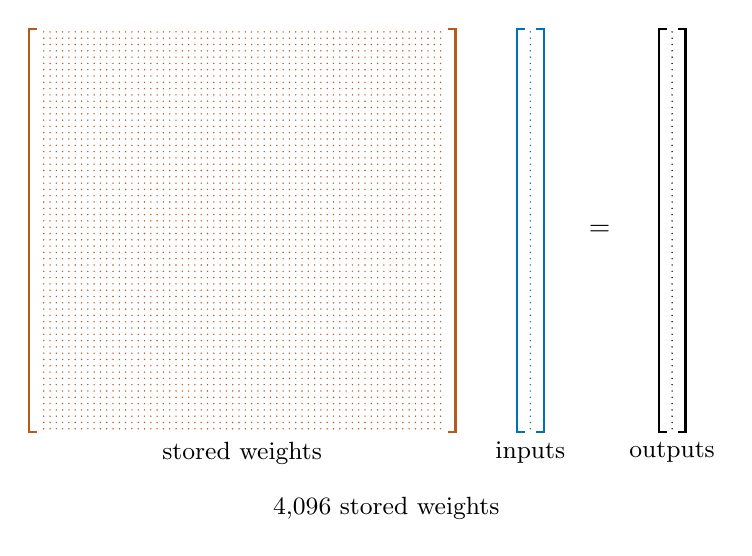
\begin{tikzpicture}[x=1mm,y=1mm,font=\small]

        % 51.2 mm / 0.8 mm = 64 dots in each direction.
        % Place every dot half a cell in from the grid boundaries.
        \foreach \row in {0,...,63} {
          \fill[copper] foreach \col in {0,...,63} {
            ({0.4+0.8*\col},{0.4+0.8*\row}) circle[radius=0.1mm]
          };
        }

        \draw[copper,thick]
        (-0.5,51.2) -- (-1.5,51.2)
        -- (-1.5,0) -- (-0.5,0);
        \draw[copper,thick]
        (51.7,51.2) -- (52.7,51.2)
        -- (52.7,0) -- (51.7,0);

        % Input vector: 64 numbers.
        \foreach \row in {0,...,63}
          \fill[blue] (62.2,{0.4+0.8*\row}) circle[radius=0.1mm];

        \draw[blue,thick]
        (61.5,51.2) -- (60.5,51.2)
        -- (60.5,0) -- (61.5,0);
        \draw[blue,thick]
        (62.9,51.2) -- (63.9,51.2)
        -- (63.9,0) -- (62.9,0);

        \node at (71,25.6) {$\slideequals$};

        % Output vector: 64 numbers.
        \foreach \row in {0,...,63}
          \fill[black] (80.2,{0.4+0.8*\row}) circle[radius=0.1mm];

        \draw[thick]
        (79.5,51.2) -- (78.5,51.2)
        -- (78.5,0) -- (79.5,0);
        \draw[thick]
        (80.9,51.2) -- (81.9,51.2)
        -- (81.9,0) -- (80.9,0);

        % Consistent labels, without braces.
        \node[below] at (25.6,0) {stored weights};
        \node[below] at (62.2,0) {inputs};
        \node[below] at (80.2,0) {outputs};

        \node[below] at (43.9,-7)
        {4,096 stored weights};

      \end{tikzpicture}
    }
  \end{overlayarea}
\end{frame}

\begin{frame}[plain,noframenumbering]
  
\begin{tikzpicture}[remember picture,overlay]

    % Copper dots cover the entire slide.
    \path[
    pattern=weightdots,
    pattern color=copper
    ]
    (current page.south west)
    rectangle
    (current page.north east);

    % Text centered on the slide, directly over the dots.
    \node[
    anchor=center,
    text width=0.70\paperwidth,
    align=center,
    inner sep=0pt
    ] at (current page.center)
    {%
      \begin{minipage}{0.70\paperwidth}
        \centering

        \uncover<2->{%
          At this scale, an AI weight matrix
          could be about\\
          \textbf{65 metres wide}.\par
          \medskip
          {\scriptsize
            $8{,}192\times8{,}192$ weights,
            on a 72-inch display.\par}
        }

        \vspace{5mm}

        \uncover<3->{%
          AI models can have \textit{trillions} of weights,\\
          requiring many trillions of operations per response.\par
        }

        \vspace{5mm}

        \uncover<4->{%
          \textit{How can we make MVM cheaper?}
        }
      \end{minipage}
    };

  \end{tikzpicture}
  \null
\end{frame}

\begin{frame}{MVM from circuit laws}
  \vspace{-5mm}
  \centering
  
  \begin{tikzpicture}[
    x=0.9cm, y=0.9cm,
    >=stealth,
    line width=0.7pt,
    circuit ee IEC,
    set resistor graphic=var resistor IEC graphic,
    scale=1.5
    ]
    \ctikzset{bipoles/resistor/height=0.15}
    \ctikzset{bipoles/resistor/width=0.4}
    \ctikzset{bipoles/thickness=0.7}

    \path[use as bounding box]
    (-1.55,-2.4) rectangle (5.85,2.8);

    \only<1-5>{
      % Input arrows and voltage labels.
      \foreach \y/\i/\start in {0/1/2,1/2/3,2/3/3} {
        \only<\start->{
          \draw[->] (-1.15,\y) -- (-0.72,\y);
          \node[left] at (-1.18,\y) {$V_{\i}$};
        }
      }

      % Wires: mutually exclusive stages.
      \only<2>{
        \draw (-0.72,0) -- (-0.4,0);
        \draw (0,-0.4) -- (0,-0.7);
        \draw[->] (0,-0.7) -- (0,-1.0);
      }

      \only<3>{
        \foreach \y in {0,1,2} {
          \draw (-0.72,\y) -- (-0.4,\y);
        }
        \draw (0,2) -- (0,-0.7);
        \draw[->] (0,-0.7) -- (0,-1.0);
      }

      \only<4>{
        \foreach \y in {0,1,2} {
          \draw (-0.72,\y) -- (1.5,\y);
        }
        \foreach \x in {0,1} {
          \draw (\x,2) -- (\x,-0.7);
          \draw[->] (\x,-0.7) -- (\x,-1.0);
        }
      }

      \only<5->{
        \foreach \y in {0,1,2} {
          \draw (-0.72,\y) -- (5.7,\y);
        }
        \foreach \x in {0,1,2,3,4,5} {
          \draw (\x,2) -- (\x,-0.7);
          \draw[->] (\x,-0.7) -- (\x,-1.0);
        }
      }

      % Current arrows on the first summing line.
      \only<3->{
        \draw[->] (0,1.42) -- (0,1.15);
        \draw[->] (0,0.42) -- (0,0.15);
      }

      % First physical column: each resistor drawn exactly once.
      \foreach \y/\i/\start in {0/1/2,1/2/3,2/3/3} {
        \only<\start->{
          \draw (-0.4,\y)
          to[/tikz/circuitikz/bipoles/length=20pt, R]
          (0,\y-0.4);
        }
        \only<\start-3>{
          \node[font=\scriptsize, inner sep=0pt, anchor=west]
          at (-0.48,\y-0.54) {$G_{\i1}$};
        }
        \only<4->{
          \node[font=\tiny, inner sep=0pt, anchor=west]
          at (-0.48,\y-0.54) {$G_{\i1}^{+}$};
        }
      }

      % Remaining physical columns.
      \foreach \x/\j/\sgn/\start in {
        1/1/-/4,
        2/2/+/5,
        3/2/-/5,
        4/3/+/5,
        5/3/-/5
      } {
        \only<\start->{
          \foreach \y/\i in {0/1,1/2,2/3} {
            \draw (\x-0.4,\y)
            to[/tikz/circuitikz/bipoles/length=20pt, R]
            (\x,\y-0.4);

            \node[font=\tiny, inner sep=0pt, anchor=west]
            at (\x-0.48,\y-0.54)
            {$G_{\i\j}^{\sgn}$};
          }
        }
      }

      % Output labels.
      \foreach \x/\j/\sgn/\start in {
        0/1/+/4,
        1/1/-/4,
        2/2/+/5,
        3/2/-/5,
        4/3/+/5,
        5/3/-/5
      } {
        \only<\start->{
          \node[below] at (\x,-1.0) {$I_{\j}^{\sgn}$};
        }
      }

      % Stage-specific explanations.
      \only<2>{
        \node[
        anchor=north west, align=left,
        inner sep=0pt, font=\small
        ] at (-0.1,-1.12)
        {$I_1=V_1G_{11}$\\(Ohm's Law)};
      }

      \only<3>{
        \node[
        anchor=north west, align=left,
        inner sep=0pt, font=\small
        ] at (-0.1,-1.12)
        {$I_1=V_{1}G_{11}+V_{2}G_{21}+V_{3}G_{31}$\\
          (Kirchhoff's Current Law)};
      }

      \only<4>{
        \node[
        anchor=north west, align=left, inner sep=0pt
        ] at (2.0,-1.12)
        {$I_{\mathrm{diff}}=I_1^+-I_1^-$\\
          (Differential pairs)};
      }

      \only<5->{
        \node[font=\small, align=center] at (2.5,-2)
        {$\displaystyle
          I_j=
          V_1\bigl(G_{1j}^{+}-G_{1j}^{-}\bigr)
          + V_2\bigl(G_{2j}^{+}-G_{2j}^{-}\bigr)
          + V_3\bigl(G_{3j}^{+}-G_{3j}^{-}\bigr)$};
      }
    }

    % ----------------------------------------------------------
    % Overlay 6: 8 rows × 18 columns of resistors.
    % ----------------------------------------------------------
    \only<6>{%
      \begin{scope}[
        shift={(2.15,0.00)},
        scale=0.5,
        transform shape,
        draw=black,
        text=black,
        line width=0.7pt
        ]
        % Center the complete array, including leads.
        \begin{scope}[shift={(-8.175,-3.0)}]

          % Input row wires and arrows.
          \foreach \y in {0,...,7} {
            \draw[->] (-1.15,\y) -- (-0.72,\y);
            \draw (-0.72,\y) -- (17.5,\y);
          }

          % Output column wires and arrows.
          \foreach \x in {0,...,17} {
            \draw (\x,7) -- (\x,-0.7);
            \draw[->] (\x,-0.7) -- (\x,-1.0);
          }

          % Resistors, drawn after the wires.
          \foreach \x in {0,...,17} {
            \foreach \y in {0,...,7} {
              \draw (\x-0.4,\y)
              to[/tikz/circuitikz/bipoles/length=20pt, R]
              (\x,\y-0.4);
            }
          }

        \end{scope}
      \end{scope}
    }

    % Overlay 7: 3 rows × 6 columns of array blocks.
    \only<7->{%
      \begin{scope}[
        shift={(2.15,0.00)},
        draw=black,
        text=black,
        line width=0.5pt
        ]

        \foreach \row in {0,...,2} {
          \foreach \col in {0,...,5} {
            \begin{scope}[
              shift={({1.3*(\col-2.5)},{1.3*(1-\row)})}
              ]

              % Square array.
              \draw (-0.30,-0.30) rectangle (0.30,0.30);

              % Four input leads.
              \foreach \offset in {-0.225,-0.075,0.075,0.225} {
                \draw (-0.52,\offset) -- (-0.30,\offset);
              }

              % Four output leads.
              \foreach \offset in {-0.225,-0.075,0.075,0.225} {
                \draw (\offset,-0.30) -- (\offset,-0.52);
              }

            \end{scope}
          }
        }

        % Continuation dots outside the grid.
        \foreach \row in {0,...,2} {
          \node[font=\scriptsize,inner sep=0pt]
          at (-4.05,{1.3*(1-\row)}) {$\cdots$};
          \node[font=\scriptsize,inner sep=0pt]
          at (4.05,{1.3*(1-\row)}) {$\cdots$};
        }

        \foreach \col in {0,...,5} {
          \node[font=\scriptsize,inner sep=0pt]
          at ({1.3*(\col-2.5)},2.10) {$\vdots$};
          \node[font=\scriptsize,inner sep=0pt]
          at ({1.3*(\col-2.5)},-2.10) {$\vdots$};
        }

      \end{scope}
    }
  \end{tikzpicture}
\end{frame}

\begin{frame}{Phase-change memory}
  \centering
  \begin{columns}[T, onlytextwidth]
    \begin{column}{0.55\textwidth}
      \begin{itemize}
      \item<1-> One weight stored as one conductance
      \item<2-> Programmed with \textit{current pulses} 
      \item<3-> Several \textit{nonidealities}
        \begin{itemize}
        \item<4-> Programming noise
        \item<5-> Read noise
        \item<6-> Device variation
        \item<7-> Drift— $G(t)=G(t_0)\left(\frac{t}{t_0}\right)^{-\nu}$
        \end{itemize}
      \end{itemize}
    \end{column}
    \begin{column}{0.45\textwidth}
      \centering
      \uncover<7->{
        \vspace{5mm}
        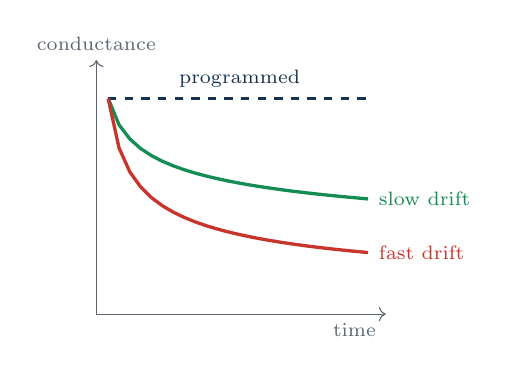
\begin{tikzpicture}[x=1cm,y=1cm,font=\scriptsize, scale=0.75, domain=0.2:4.6]
          \draw[->,muted] (0,0)--(4.9,0) node[below left]{time};
          \draw[->,muted] (0,0)--(0,4.3) node[above]{conductance};
          \draw[navy,very thick,dashed] (0.2,3.65)--(4.65,3.65)
          node[midway,above]{programmed};
          \draw[good,very thick] plot (\x, {3.65 * pow(\x/0.2, -0.2)})
          node[right]{slow drift};
          \draw[bad,very thick] plot (\x, {3.65 * pow(\x/0.2, -0.4)})
          node[right]{fast drift};
        \end{tikzpicture}
      }
    \end{column}
  \end{columns}
\end{frame}

\begin{frame}{Tolerating drift}
  \begin{itemize}
  \item<1-> Different ways of representing $\vec{y}=A\vec{x}=(A^+-A^-)\vec{x}$
  \end{itemize}
  \par\vspace{3mm}
  \small {
    \renewcommand{\arraystretch}{1.5}
    \begin{tabular}{@{}>{\raggedleft\color{navy}}m{65mm}!{\color{copper}\vrule width 1pt\hspace{0mm}}>{\raggedright\arraybackslash}m{100mm}@{}}
      \uncover<2->{Offset weights on differential pairs&$\vec{y}=[(A^++B)-(A^-+B)]\vec{x}$}\\
      \uncover<3->{Permutations of rows and columns&$\vec{y}=P^{-1}AP\vec{x}$}\\
      \uncover<4->{Scaled weights with compensation&$\vec{y}=\frac{1}{s}(s A) \vec{x}$}
    \end{tabular}
  }
  \begin{itemize}
  \item<5-> These diverge under drift.
  \item<6-> Pick $B$, $P$, $s$ to minimize error over time.
  \item<7-> \textbf{More general}: optimize each conductance individually
  \end{itemize}
\end{frame}

\begin{frame}{Optimization loop}
  \centering
  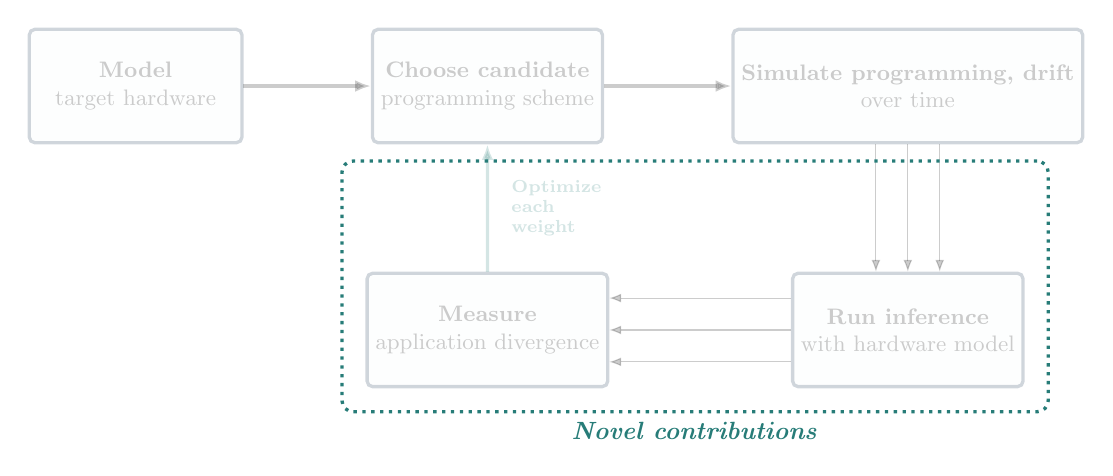
\begin{tikzpicture}[
    font=\small,
    node distance=6mm,
    b/.style={
      rounded corners=2pt,
      draw=navy,
      very thick,
      fill=pale,
      minimum width=30mm,
      minimum height=16mm,
      align=center
    },
    h/.style={
      b,
      fill=warm
    },
    a/.style={
      -{Latex[length=2mm]},
      very thick
    }
    ]

    \begin{scope}[scale=0.9, transform shape]

      % ============================================================
      % Hardware characterization -- revealed on slide 1
      % ============================================================
      \node[
      b,
      opacity=.2,
      onslide=<2-5>{opacity=.6},
      onslide=<1>{opacity=1},
      onslide=<6>{opacity=1}
      ] (char) {%
        \textbf{Model}\\
        target hardware
      };

      % ============================================================
      % Choose candidate -- revealed on slide 2
      % ============================================================
      \node[
      b,
      right=18mm of char,
      opacity=.2,
      onslide=<3-5>{opacity=.6},
      onslide=<2>{opacity=1},
      onslide=<6>{opacity=1}
      ] (choose) {%
        \textbf{Choose candidate}\\
        programming scheme
      };

      % ============================================================
      % Simulate programming / drift -- revealed on slide 3
      % ============================================================
      \node[
      b,
      right=18mm of choose,
      opacity=.2,
      onslide=<4-5>{opacity=.6},
      onslide=<3>{opacity=1},
      onslide=<6>{opacity=1}
      ] (drift) {%
        \textbf{Simulate programming, drift}\\
        over time
      };

      % ============================================================
      % Run inference -- revealed on slide 4
      % ============================================================
      \node[
      b,
      below=18mm of drift,
      opacity=.2,
      onslide=<5>{opacity=.6},
      onslide=<4>{opacity=1},
      onslide=<6>{opacity=1}
      ] (comp) {%
        \textbf{Run inference}\\
        with hardware model
      };

      % ============================================================
      % Application divergence -- revealed on slide 5
      % ============================================================
      \node[
      b,
      below=18mm of choose,
      opacity=.2,
      onslide=<6>{opacity=1},
      onslide=<5>{opacity=1}
      ] (loss) {%
        \textbf{Measure}\\
        application divergence
      };

      % ============================================================
      % Enter loop -- revealed on slide 2
      % ============================================================
      \draw[
      a,
      opacity=.2,
      onslide=<3-5>{opacity=.6},
      onslide=<2>{opacity=1},
      onslide=<6>{opacity=1}
      ] (char) -- (choose);

      % ============================================================
      % Top edge -- revealed on slide 3
      % ============================================================
      \draw[
      a,
      opacity=.2,
      onslide=<4-5>{opacity=.6},
      onslide=<3>{opacity=1},
      onslide=<6>{opacity=1}
      ] (choose) -- (drift);

      % ============================================================
      % Right edge -- revealed on slide 4
      % ============================================================
      \foreach \x in {-0.25,0,0.25} {
        \draw[
        -{Latex[length=1.5mm]},
        opacity=.2,
        onslide=<5>{opacity=.6},
        onslide=<4>{opacity=1},
        onslide=<6>{opacity=1}
        ]
        ([xshift=-\x*18mm]drift.south) --
        ([xshift=-\x*18mm]drift.south |- comp.north);
      }

      % ============================================================
      % Bottom edge -- revealed on slide 5
      % ============================================================
      \foreach \y in {-0.25,0,0.25} {
        \draw[
        -{Latex[length=1.5mm]},
        opacity=.2,
        onslide=<6>{opacity=1},
        onslide=<5>{opacity=1}
        ]
        ([yshift=-\y*18mm]comp.west) --
        ([yshift=-\y*18mm]comp.west -| loss.east);
      }

      % ============================================================
      % Feedback arrow -- revealed on slide 6
      % ============================================================
      \draw[
      -{Latex[length=2mm]},
      very thick,
      draw=teal,
      opacity=.2,
      onslide=<5-6>{opacity=1}
      ]
      (loss.north)
      -- (choose.south)
      node[
      midway,
      right=2mm,
      text=teal,
      font=\scriptsize\bfseries,
      align=left
      ] (optimize) {%
        Optimize\\
        each\\
        weight
      };

      % Novel contributions -- visible only on the final overlay.
      % "overlay" prevents the box from changing the diagram's layout.
      \only<6>{%
        \node[
        overlay,
        fit={
          (loss)
          (optimize.south west)
          (optimize.south east)
          ([yshift=-2mm]optimize.north)
          (comp)
        },
        draw=teal,
        very thick,
        dotted,
        rounded corners=4pt,
        inner sep=3mm,
        label={
          [text=teal, font=\bfseries]
          below:\textit{Novel contributions}
        }
        ] {};
      }

    \end{scope}
  \end{tikzpicture}
\end{frame}

\end{document}
